\chapter{Hardvér}

\label{kap:hardver}

V tejto kapitole popíšeme a rozoberieme niektoré aspekty zvoleného hardvéru, ktoré sú podstatné pre účely tejto práce.

Pri útokoch pomocou indukovania chýb je často potrebná vysoká presnosť časovania v stovkách až desiatkach nanosekúnd. Lacnejší hardvér často takúto presnosť nie je schopný dosiahnuť. Hlavným cieľom tejto práce je overiť túto skutočnosť a zistiť akú presnosť časovania dokáže takýto hardvér poskytnúť. Finančné náklady na všetky súčiastky použité pri implementovaných útokoch sa pohybujú rádovo v desiatkach eúr.

\section{ATMega328P}
Najdôležitejším zariadením pre účely tejto práce je Atmel mikrokontrolér s 8-bitovou architektúrou AVR, dnes pod firmou Microchip Technology. Tento mikrokontrolér je súčasťou viacerých modelov vývojových dosiek Arduino, ktoré sú často využívané pri vývoji jednoduchých vnorených zariadení. Zároveň zvykne byť použitý aj pri nasadení skutočných produktov, najmä vnorených systémov s nízkou spotrebou. Mikrokontrolér ATMega328P bol aj preto zvolený ako cieľom útokov implementovaných v tejto práci, ale hlavným dôvodom bola jeho veľmi nízka cena pohybujúca sa okolo desať eúr. Techniky útokov použité v tejto práci môžu s nezanedbateľnou pravdepodobnosťou trvalo poškodiť cielený hardvér, preto sme sa rozhodli použiť viacej rovnakých čipov. Konkrétne boli testované štyri exempláre formátu ATMega328P-PU z dvoch (po dvojiciach) rôznych sérií výroby (2139E4A a 2128BQY). Okrem toho bol použitý aj ako zdroj generujúci riadiace impulzy do rôznych obvodov využívajúcich niektoré techniky útokov spomenuté v kapitole \ref{kap:teoria}. Pre tento druhý účel bol použitý ako súčasť dosky Arduino Nano.

\subsection{Kľúčové vlastnosti}
Zvolený formát čipu ATMega328P-PU je v púzdre THT (Through Hole Technology), čo znamená, že vonkajšie piny na čipe sú vyvedené vo forme \uv{kolíkov} a je možné čip zapojiť bez potreby pájkovania pomocou nepájivého kontaktného poľa (angl. solderless breadboard). Takéto zapojenie potom možno jednoducho a bezprostredne modifikovať počas experimentovania. Ďalšou vlastnosťou je možnosť pripojenia externého oscilátora s frekvenciou maximálne 16 MHz, čo znamená väčšiu flexibilitu nastaviteľných parametrov jednotlivých útokov. Na čipe sa nachádza aj interný oscilátor s frekvenciou 8 MHz a možno ho využiť miesto zapojenia s externým \cite{atmegaData}.

Čo sa týka softvéru, pre programovanie mikrokontroléra ATMega328P je potrebný kompilátor nízko-úrovňového jazyka (napríklad C) pre architektúru AVR. Nahratie programu do trvácnej flash-pamäte na mikrokontroléri možno zabezpečiť napríklad pomocou ISP (In-System Programming) programátora. Pre tento účel, je potrebné, aby na mikrokontroléri bol prítomný zavádzací program (angl. bootloader), ďalej len zavádzač, ktorý dokáže komunikovať s ISP programátorom. Jednoduchý a automatizovaný spôsob pre vykonanie týchto operácií poskytuje aj integrované vývojové prostredie (IDE) Arduino IDE, ktoré sme sa rozhodli použiť. Arduino IDE interne používa kompilátor AVR-GCC a ISP programátor AVRDUDE, ktoré sú voľne dostupné aj samostatne.

\subsection{Architektúra AVR}
Mikrokontrolér ATMega328P implementuje osem bitovú architektúru AVR. Niektoré aspekty tejto architektúry sú dôležité pre pochopenie niektorých častí kódu písaných v asembleri v rámci tejto práce, preto ich stručne opíšeme. AVR je zaraďovaná do triedy RISC (Reduced Instruction Set Computer) architektúr \cite{avrInstruction}. Poskytuje tridsaťdva (R0 -- R31) 8-bitových všeobecných registrov, z nich niektoré so špeciálnym významom pri vybraných inštrukciách. V tejto práci používame tieto registre len v základnom, všeobecnom význame. Pre prístup do pamäte slúžia dve základné inštrukcie LD (Load) a ST (Store), prípadne ich varianty. 

Ovládanie GPIO (General Purpose Input Output) pinov na mikrokontroléri je zabezpečené pomocou špeciálnych vstupno-výstupných registrov. Každý pin je súčasťou jedeného zo štyroch tzv. portov (ozn. A -- D) a v rámci portu má priradený jeden z ôsmich bitov (0 -- 7). Každý pin je potom ovládaný troma registrami DDRX, PINX a PORTX, kde X je písmeno označujúce port priradený pinu. Bit pinu potom určuje index konkrétneho bitu (0 označuje najmenej významný bit) v týchto troch registroch (rovnaký index pre každý register), ktorým možno ovládať daný pin. Význam jednotlivých bitoch v registroch je potom nasledovný: DDR (Data Direction register) určuje smer toku dát, pokiaľ je príslušný bit v tomto registri nastavený na 0, pin je vo vstupnom móde, pokiaľ je nastavený na 1, pin je vo výstupnom móde. Register PIN má význam vo vstupnom móde a v danom bite udržiava logickú hodnotu vstupu na danom pine. Register PORT má naopak hlavný význam vo výstupnom móde a hodnota v príslušnom bite je výstupnou logickou hodnotou na priradenom pine. Tieto vstupno-výstupné registre možno adresovať priamo pomocou vyhradeného adresného priestoru v pamäti (memory-mapped I/O), alebo s využitím špeciálnych inštrukcií (port-mapped I/O).

Pre lepšie porozumenie uvedieme príklad. Chceme nastaviť digitálny pin 13 ako výstupný a na výstupe chceme periodicky prepínať medzi logickými hodnotami 0 a 1, napríklad s účelom blikať LED diódou, ďalej len LED (Light Emitting Diode). GPIO pin 13 má priradený port B, bit 5. Potrebujeme preto nastaviť v registeri DDRB bit 5 na 1, čím nastavíme pin do výstupného módu. Následné prepínaním medzi hodnotami 0 a 1 v registri PORTB (bit 5) dosiahneme želaný efekt na GPIO pine 13. Nastavenie hodnoty konkrétneho bitu vo vstupno-výstupnom registri možno docieliť napríklad pomocou vstupno-výstupných inštrukcií SBI (Set Bit in I/O Register) a CBI (Clear Bit in I/O register), ktoré nastavia daný bit na 1 resp. 0 \cite{avrInstruction}. Tieto inštrukcie používajú vstupno-výstupné adresy daných registrov, ktoré v našom prípade sú 0x04 (DDRB) a 0x05 (PORTB) \cite{atmegaData}. Ukážky jednotlivých inštrukcií v jazyku asembler sa nachádzajú v tabuľke \ref{tab:ovladanieVV}. V prípade, že by sme chceli hodnoty v registroch nastaviť pomocou inštrukcií LD a ST (prípadne ich variánt), použili by sme adresy týchto registrov v mape pamäti -- 0x24, resp. 0x25 \cite{atmegaData}.

\begin{table}
    \caption[Ovládanie vstupno-výstupných registrov na architektúre AVR]{Ovládanie vstupno-výstupných registrov na architektúre AVR.}
    \label{tab:ovladanieVV}
    \begin{center}
    \begin{tabular}{|c|c|}
        \hline 
        Inštrukcia & Komentár \\
        \hline
        sbi 0x04, 5 & nastavenie bitu 5 na 1 v registri DDRB \\
        \hline
        sbi 0x05, 5 & nastavenie bitu 5 na 1 v registri PORTB \\
        \hline
        cbi 0x05, 5 & nastavenie bitu 5 na 0 v registri PORTB \\
        \hline
    \end{tabular}
    \end{center}
\end{table}

\subsection{Základné zapojenie mikrokontroléra}
V tejto časti predstavíme zapojenie mikrokontroléra ATMega328P-PU, ktoré neskôr využijeme pri implementácií vybraných útokov v kapitole \ref{kap:utoky}. Zapojenie spočíva v pripojení súčiastok, ktoré zabezpečujú základné funkcie mikrokontroléra, konkrétne pripojíme zdroj napätia, externý oscilátor, tlačidlo pre hardvérový reštart, prevádzanie signálu medzi protokolmi USB (Universal Serial Bus) a UART (Universal Asynchronous Receiver-Transmitter) pre komunikáciu s počítačom a LED k portu B, bitu 5, ktorú používa zavádzač na signalizáciu prebiehajúcej komunikácie. Pripojenú LED možno zároveň využiť na výstupné signály aj v samotnom programe nahratom na mikrokontroléri. Zoznam a popis všetkých použitých súčiastok:
\begin{itemize}
    \item ATMega328P-PU -- THT púzdro, umožňuje použiť kontaktné nepájivé pole
    \item prevodník medzi USB a UART -- použitý modul s čipom CP2102, na doske je vyvedený aj výstup z napájania pomocou USB
    \item kontaktné nepájivé pole -- umožňuje flexibilne prepájať súčiastky bez potreby spájkovania
    \item spínacie tlačidlo -- po stlačení uzemní RST pin, čo vynúti reštart mikrokontroléra
    \item 16 MHz kryštál -- pre zapojenie externého oscilátora
    \item keramické kondenzátory -- 2-krát 22 pF záťažové kondenzátory ku kryštálu, 1-krát 0.1 \textmu F pre využitie DTR pinu
    \item rezistory -- 1-krát 330 $\Omega$ k LED, 1-krát 10k $\Omega$ -- zdvíhací odpor RST pinu
    \item LED dióda -- použili sme žltú farbu a veľkosť 3 mm
    \item prepojovacie kábliky typu M-M (Male to Male)
\end{itemize}
Súčiastky zapojíme podľa schémy na obrázku \ref{obr:schemeATMega}. Prevodník medzi USB a UART možno okrem bežnej sériovej komunikácie použiť aj na naprogramovanie mikrokontroléra pomocou ISP programátora, za predpokladu, že mikrokontrolér obsahuje zavádzač. Pre tento účel pripájame k RST pinu na mikrokontroléri cez kondenzátor pin DTR (Data Terminal Ready) na prevodníku. To umožní automaticky vyvolať reštart na mikrokontroléri, čo je potrebné vykonať vždy pred nahratím nového programu na mikrokontrolér. Po opätovnom zapnutí sa na krátky čas (približne sekunda) spustí zavádzač na mikrokontroléri, čo umožňuje komunikáciu s ISP programátorom. Komunikáciu so zavádzačom je potrebné iniciovať v rámci tohto časového okna, v opačnom prípade zavádzač spustí program nahratý vo flash pamäti mikrokontroléra a bude potrebné pre komunikáciu so zavádzačom mikrokontrolér opätovne reštartovať. Zvolené vývojové prostredie Arduino IDE nám umožňuje automatizovane využívať túto funkcionalitu.

\begin{figure}
    \centerline{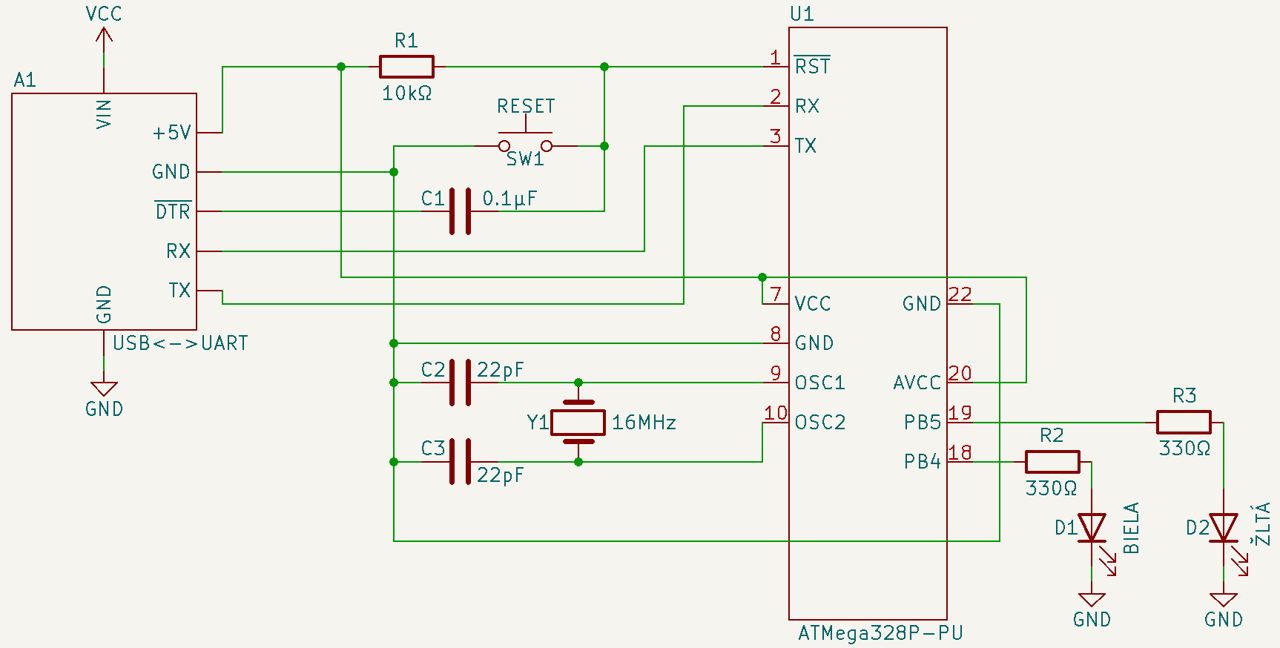
\includegraphics[width=1\textwidth]{images/schemeATMega.png}}
    \caption[Schéma zapojenia mikrokontroléra ATMega328P]{Schéma zapojenia mikrokontroléra ATMega328P.}
    \label{obr:schemeATMega}
\end{figure}

\section{STM32}
Ďalším zariadením, ktoré sme sa rozhodli použiť je mikrokontrolér z rodiny STM32, konkrétne model STM32F407, ktorý je súčasťou vývojovej dosky STM32 F4 Discovery. STM32 má v porovnaní s ATMega328P viacero výhod. Najpodstatnejším rozdielom pre účely tejto práce je väčšia frekvencia procesora, ktorá je dokonca nastaviteľná interným PLL obvodom. Maximálna hodnota je 168 MHz, čo je značne väčšia frekvencia oproti 16 MHz na ATMega328P. Dosku STM32 F4 Discovery sme sa preto rozhodli použiť ako alternatívu k Arduino Nano, pre účel generovania riadiacich impulzov do obvodov indukujúcich chyby na cieľovom zariadení. Pri použití STM32 preto očakávame väčšiu presnosť pri načasovaní útoku. Ďalšími výhodami sú napríklad väčší výkon procesora, viac vstupno-výstupných pinov a väčšia kapacita pamäte, za cenu o niečo väčšej spotreby. Tieto aspekty však nie sú významné pre cieľ tejto práce.

Dosku STM32 F4 Discovery sme sa rozhodli programovať pomocou integrovaného vývojového prostredia STM32CubeIDE, ktoré je odporúčané aj výrobcom dosky. Prostredie poskytuje viacero užitočných funkcionalít. Podstatné pre nás bolo grafické rozhranie pre konfiguráciu vstupu a výstupu na mikrokontroléri a automatické generovanie kódu, ktorý túto konfiguráciu pri inicializácií nastaví. Takýto prístup značne zjednodušil konfiguráciu vstupno-výstupného hardvéru, ktorá je na mikrokontroléroch STM32 zložitejšia v porovnaní s ATMega328P.

\subsection{Architektúra STM32 Cortex-M4}
Mikrokontroléry STM32 sú založené na 32-bitovej Arm Cortex-M RISC architektúre. Nami použitý model STM32F407 implementuje architektúru STM32 Cortex-M4. Predstavíme niektoré aspekty tejto architektúry a rozdiely z architektúrou AVR podstatné pre túto prácu. K dispozícii je 13 32-bitových všeobecných registrov (R0--R12). Registre R13 (SP -- Stack Pointer), R14 (LR -- Link Register) majú špeciálny význam pri volaní procedúr \cite{stmInstruction} a nebudeme ich v tejto práci používať. Register R15 (PC) obsahuje adresu nasledovnej inštrukcie, rovnako ako vo väčšine architektúr. Pre prístup do pamäte možno použiť inštrukcie (prípadne varianty) LDR (Load) a STR (Store), podobne ako v architektúre AVR.

GPIO piny možno obdobne ovládať pomocou vstupno-výstupných registrov, pričom v porovnaní s architektúrou AVR je mierne odlišné. Vonkajšie piny majú opäť priradený port, tentokrát z väčšieho rozsahu (ozn. GPIOA--GPIOK), a bit priradený z rozsahu 0 -- 15. Všetky vstupno-výstupné registre sú 32-bitové, preto v niektorých má pin priradené 2 bity, ktoré môžu mať rôzny význam \cite{stmReference}. Týchto registrov, ktoré ovládajú piny priradené do jedného GPIO portu je v porovnaní s AVR architektúrou výrazne viac, predstavíme preto len tie, ktoré sme v práci priamo použili. Register GPIOX\_IDR (Input Data register), kde X je písmeno portu (A--K), má význam vo vstupnom móde pinu. Spodné bity (0--15) obsahujú logickú hodnotu na vstupe príslušných pinov priradeným týmto bitom. Vrchné bity (16--31) v týchto registroch sú rezervované a musia mať nastavenú hodnotu nula \cite{stmReference}. Register GPIOX\_BSRR (Bit Set/Reset Register) možno použiť pre atomické nastavenie logickej hodnoty na výstupnom pine. Register je určený iba pre zápis (čítanie vráti vždy 0x0000). Nastavenie príslušného bitu na 1 v spodnej časti registra (bity 0--15) spôsobí následovné nastavenie logickej hodnoty 1 na výstupe. Naopak nastavenie bitu na 1 vo vrchnej časti registra (bit 16--31 ovláda pin s priradeným bitom 0--15) spôsobí nastavenie logickej hodnoty 1 na výstupe. Nastavenie ktoréhokoľvek bitu na 0 v tomto registri nemá žiaden vplyv na stav GPIO pinu. Piny vo Výstupnom móde možno ovládať aj pomocou ďalších registrov. Výhoda spomenutého prístupu je možnosť atomického nastavenia viacerých pinov naraz po zápise hodnoty do registra GPIOX\_BSRR. Pre ovládanie a konfiguráciu GPIO pinov v architektúre STM32 CORTEX-M4 je potrebné nastaviť ďalšie vstupno-výstupné registre, tie sme však v tejto práci nenastavovali priamo na úrovni jazyku asembler, ale použili sme funkciu prostredia STM32CubeIDE, ktoré dokáže automatizovane vygenerovať potrebný kód v jazyku C, preto ich nebudeme uvádzať.

Adresovanie vstupno-výstupných portov v tejto architektúre je možné len prostredníctvom im vyhradených adries v pamäti, pomocou inštrukcií LDR a STR. Tento pamäťový priestor je organizovaný podľa portov. Každý port (GPIOA--GPIOK) začína na pevnej bázovej adrese a každý typ GPIO registrov má určený ofset od tejto adresy. Adresa konkrétneho GPIO registra v rámci portu je potom súčet bázovej adresy portu a ofsetu typu registra. Niekedy je vhodné uložiť hodnotu bázovej adresy do všeobecného registra. S využitím tohto registra sa potom môžeme nepriamou adresáciou s doplnkom (pomocou inštrukcie LDR) odkazovať na jednotlivé registre daného portu. Uloženie konštanty nie je vždy možné pomocou inštrukcie MOV, keďže tá obmedzuje možné hodnoty konštánt, ktoré možno použiť v druhom operande \cite{stmInstruction}. Dôvodom obmedzenia je počet bitov (12) vyhradený pre zakódovanie konštanty v strojovom kóde. Alternatívny spôsob pre uloženie ľubovolnej 32-bitovej konštanty do registra bez obmedzení je využitie takzvaného bloku literálov (angl. literal pool), pomocou pseudoinštrukcie asemblera. Ten takúto inštrukciu nahradí alokovaním špeciálneho priestoru v pamäti medzi inštrukciami na vhodnom mieste, na ktoré uloží túto konštantu. Následne pomocou inštrukcie LDR a relatívneho adresného módu k registru PC uloží konštantu z tohto miesta do registra, ktorý je cieľovým operandom pseudoinštrukcie. V algoritme \ref{alg:stmAsm} uvádzame príklad použitia takejto pseudoinštrukcie a ovládanie výstupnej hodnoty na pine pomocou GPIO portov.

\begin{lstlisting}[float,language=C,caption={Nastavenie hodnoty výstupneho pinu GPIOD 9 na STM32F4 v jazyku asembler. Pre uloženie bázovej adresy portu GPIOD použijeme blok literálov.}, label=alg:stmAsm]
; ulozenie bazovej adresy GPIOD do r0 pomocou bloku literalov
LDR r0, =#40020C00

; nastavenie pinu na logicku 1 pomocou GPIOD_BSRR (ofset 0x18)
MOV r1, #0x200 
STR r1, [r0, #0x18] 

; nastavenie pinu na logicku 0 pomocou GPIOD_BSRR (ofset 0x18)
MOV r1, #0x2000000
STR r1, [r0, #0x18]
\end{lstlisting}

\section{Ďalšie zariadenia a pomocné súčiastky}
Okrem spomenutých mikrokontrolérov sme použili aj ďalší podporný hardvér, ktorý v tejto časti stručne opíšeme.

\subsection{Osciloskop MDO4104C}
Dôležitým pomocným zariadením, ktoré sme v tejto práci použili je laboratórny osciloskop MDO4104C. Našim primárnym použitím tohto osciloskopu bola podrobná analýza hladiny napätia medzi významnými časťami zapojenia počas priebehu útoku. Vďaka tomu bolo možné pozorovať stav zariadení počas útoku a následne tomu prispôsobovať útočiaci hardvér, prípadne aj časti softvéru. Osciloskop dokáže merať napätie v čase s pomerne vysokou presnosťou (desiatky až stovky nanosekúnd), čo nám pomohlo pri určení presnosti načasovania, ktorú sa počas útokov podarilo dosiahnuť. Zároveň poskytuje funkciu automaticky počítať priemer viacerých meraní za sebou (počet je nastaviteľný). Následne zobrazí priemerný výsledok meraní, ktorý dynamicky aktualizuje s ďalšími meraniami.

\subsection{Bipolárne (BJT) tranzistory}
Tranzistory sú vo všeobecnosti základným stavebným kameňom všetkých integrovaných obvodov v elektronike. Bipolárny tranzistor (BJT, angl. Bipolar Junction Transistor) má tri elektródy, bázu (B), emitor (E) a kolektor (C). Pomocou napätia medzi bázou a emitorom možno ovládať prechodnosť medzi kolektorom a emitorom. Keď medzi bázu a emitor privedieme dostatočné napätie (závisí od použitého tranzistora, zvyčajne okolo 0.6 V), tranzistor sa otvorí a medzi kolektorom a emitorom môže tiecť prúd. Tento princíp v práci využijeme na útok technikou zmeny napätia. Pomocou tranzistora budeme ovládať napájanie na mikrokontroléri ATMega328P využitím riadiacich signálov do bázy tranzistora generovaných ďalším mikrokontrolérom.

\subsection{Hradlový ovládač TC4420}
Ďalší hardvérový komponent, ktorého využitie na útoky sme analyzovali je hradlový ovládač TC4420. Hradlový ovládač (angl. gate driver) je integrovaný obvod, ktorý sa používa na ovládanie zariadení s veľkým výkonom, napr. motory, pomocou zariadení s rádovo nižším výkonom ako napríklad mikroprocesorové systémy. Pomocou hradlových ovládačov možno pomocou riadiacich signálov prepínať napätie na iných súčiastkach v obvode. Túto funkcionalitu preto použijeme (podobne ako v prípade tranzistora) na útok zmenou napätia tak, že budeme pomocou tohto obvodu spínať a odopínať napätie na cieľovom ATMega328P. Keďže integrovaný obvod je kompaktný a obsahuje vnútri všetky potrebné súčiastky, jeho zapojenie je priamočiare a nevyžaduje žiadne ďalšie komponenty.